\documentclass[12pt]{article}
\usepackage{amsmath}
\usepackage{graphicx}
\usepackage{hyperref}
\usepackage[utf8]{inputenc}
\usepackage[T1]{fontenc}
\usepackage[polish]{babel}
\usepackage{scalerel}
\usepackage{changepage}


%\DeclareMathSizes{12}{20}{16}{12}

\author{Aleksander Głowacki}
\title{Sprawozdanie nr 4}
\date{10.12.2022}

\begin{document}

\maketitle

\tableofcontents

\section{Zadanie 1.}


\subsection{Opis problemu}
Wyznaczenie ilorazów różnicowych N-tych rzędów funkcji na podstawie zadanych węzłów i wartośći funkcji w tych węzłach.
Ilorazy różnicowe kolejnych rzędów odpowiadają współczynnikom wialomianu w postaci Newtona.
Wartość ta opisuje przyrost wartości funkcji na badanym przedziale.
Celem jest otrzymanie listy postaci:
\begin{center}
    $[f[x_0,x_1], f[x_0,x_1,x_2],...,f[x_0,...x_n]]$
\end{center} 
\subsection{Sposób rozwiązania}
Rozwiązanie opiera się na rekurencyjnej zależności ilorazów różnicowych wyższych rzędów:
\begin{center}
    $f[x_i] = f(x_i)$ \newline
    $f[x_0,...,x_n] = \frac{f[x_1,...,x_n] - f[x_0,...,x_{n-1}]}{x_n - x_0}$
\end{center}

\section{Zadanie 2.}

\subsection{Opis problemu}

Wykorzystanie uogólnionego algorytmu Hornera w celu obliczenia wartości wielomianu stopnia n postaci Newtona w zadanym punkcie.
Program na wejściu otrzymuje listę węzłów i ilorazów różnicowych obliczonych w poprzednim zadaniu. Działa w czasie liniowym od stopnia wielomianu.
\subsection{Sposób rozwiązania}
Obliczenie wartości wielomianu w punkcie t korzystając z postaci Newtona, gdzie znamy węzły $x_j$ i współczynniki $a_i$ - ilorazy różnicowe.
\begin{center}
    $w(t) = a_0 + \sum_{i = 1}^{n} a_i \prod_{j = 0}^{i-1} (t - t_j)$
\end{center}
Algorytm ten jest liniowy, ponieważ w kazdej iteracji pojedynczej pętli sumowania wykonuje sie tylko jedno mnożenie, gdyż korzystamy z wyniku mnożenia z poprzednjej iteracji.

\section{Zadanie 3.}

\subsection{Opis problemu}
Przekształcenie wielomianu postaci Newtona na postać naturalną, gdy zadany jest wektor węzłów i ilorazów różnicowych.
\subsection{Sposób rozwiązania}
W wielomianie interpolacyjnym, współczynnik $a_n$ przy najwyższej potędze $x_n$ jest równy cn wartości ilorazu różnicowego dla najwyższego rzędu. 
Dzięki temu możemy wyliczyć wszystkie współczynniki wielomianu zaczynając od najwyższych potęg i 
aktualizując współczynniki przy niższych potęgach, tak aby były one w postaci naturalnej. 
W kolejnych iteracjach będziemy korzystać z już obliczonych "częściowych" współczynników. Najniższy współczynnik jest sumą współczynników postaci Newtona
rozbitą po ilorazach różnicowych kolejnych rzędów. Czynnik $a_{n-1}$ występuje tylko przy ilorazie rzędu $n$ i $n-1$. Wyliczając go na tych dwóch węzłach jednocześnie 
liczymy fragment czynnika $a_{n-2}$, którego reszta skrywa się w ilorazie rzędu $n-2$. 
Stąd podwójna pętla w algorytmie - wewnątrz liczymy fragmenty wszystkich współczynników postaci 
naturalnej na bazie ilorazu różnicowego najwyższego rzędu, a w zewnetrznej petli zschodzimy do ilorazu niższego rzędu i doliczamy resztę współczynników, pomijając 
ten stojący przy najwyższej potędze, bo jest on już gotowy.
\subsection{Wnioski}
Obliczenie postaci naturalnej wielomianu, ktory interpoluje funkcję daje pewną korzyść. 
Gdy nie znamy jawnego wzoru, jedynie
wartości w określonych wezłach, trudno jest znaleźć funkcję pierwotną
potrzebną do całkowania przedziału - obliczenia pola pod wykresem funkcji.
Natomiast całkowanie wielomianu otrzymanego za pomoca ilorazów różnicowych jest trywialne, co uprascza problem i uzyskujemy przybliżoną przez wielomian wartość całki oznaczonej danej funkcji.

\section{Zadanie 4.}

\subsection{Opis problemu}
Program ma interpolować zadaną funkcję na przedziale przy pomocy wielomianu o zadanym stopniu.
\subsection{Sposób rozwiązania}
\begin{enumerate}
    \item Konstrukcja wielomianu postaci Newtona przy pomocy obliczenia ilorazów różnicowych na zadanych wężlach.
    \item Utworzenie gęstej siatki punktów na przedziale.
    \item Obliczenie wartości wielomianu w punktach.
\end{enumerate}

\section{Zadanie 5.}

\subsection{Opis problemu}
Sprawdzenie funkcji do rysowania wielomianu interpolacyjnego na następujących przykladach:
\begin{enumerate}
    \item $e^x,\hspace{0.2cm} [0,1],\hspace{0.2cm} n = 5, 10, 15$
    \item $x^2 * sin(x),\hspace{0.2cm} [-1,1],\hspace{0.2cm} n = 5, 10, 15$
\end{enumerate}
\newpage
\subsection{Wyniki}

\begin{figure}[h!]
    \caption{$e^x$ na 5 węzłach}
    \centering
    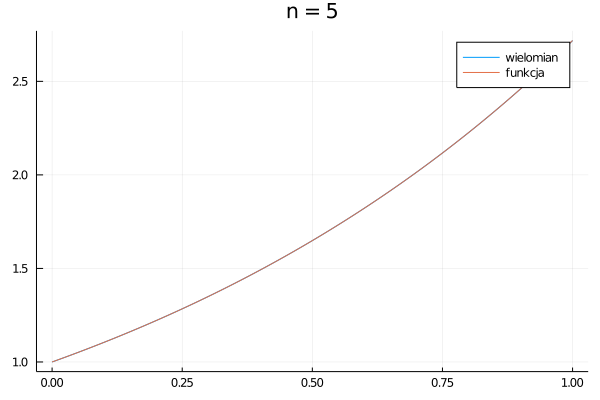
\includegraphics[scale=0.5]{z5f_5.png}
\end{figure}

\begin{figure}[h!]
    \caption{$e^x$ na 10 węzłach}
    \centering
    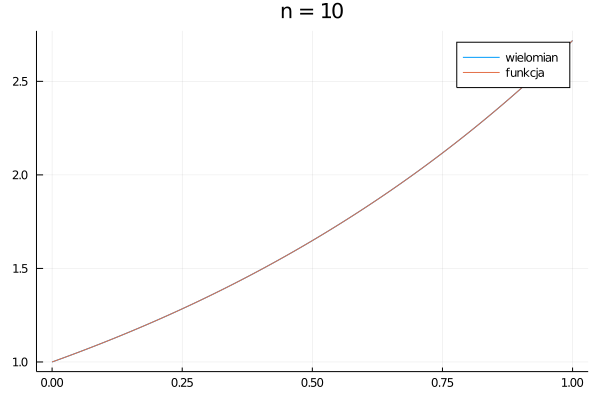
\includegraphics[scale=0.5]{z5f_10.png}
\end{figure}
\begin{figure}[h!]
    \caption{$e^x$ na 15 węzłach}
    \centering
    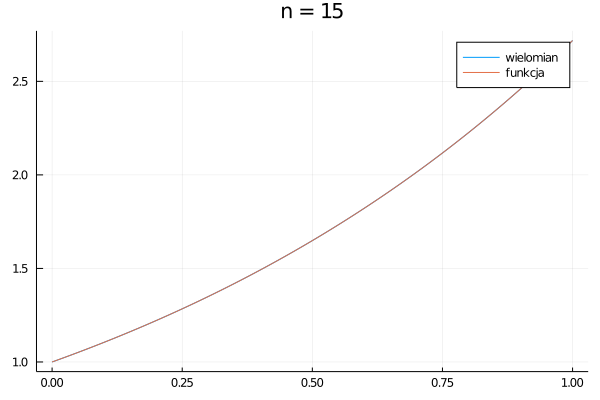
\includegraphics[scale=0.5]{z5f_15.png}
\end{figure}

\begin{figure}[h!]
    \caption{$x^2 * sin(x)$ na 5 węzłach}
    \centering
    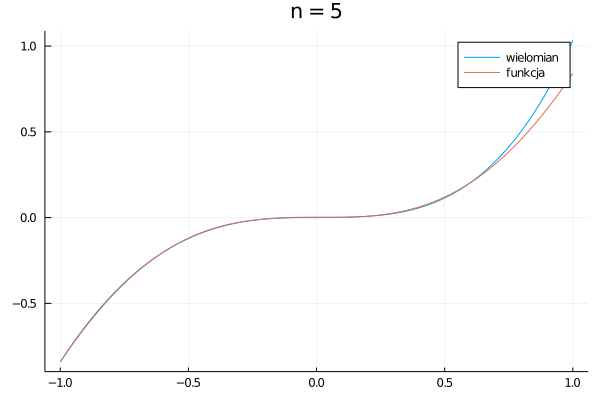
\includegraphics[scale=0.5]{z5g_5.png}
\end{figure}

\begin{figure}[h!]
    \caption{$x^2 * sin(x)x$ na 10 węzłach}
    \centering
    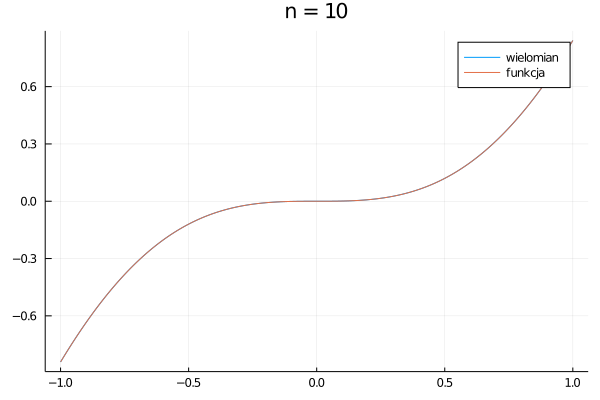
\includegraphics[scale=0.5]{z5g_10.png}
\end{figure}
\begin{figure}[h!]
    \caption{$x^2 * sin(x)$ na 15 węzłach}
    \centering
    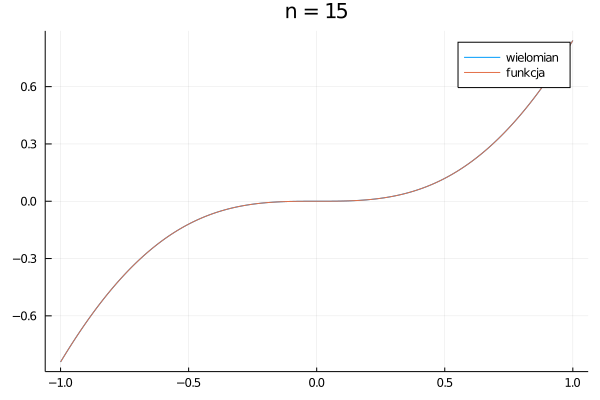
\includegraphics[scale=0.5]{z5g_15.png}
\end{figure}


\subsection{Wnioski}
Wielomian dobrze interpoluje zadane funkcje na przedziałach.
Dzieje się tak, ponieważ zadane funkcje są ciągłe, a także ich pochodne są ciągłe.

\section{Zadanie 6.}

\subsection{Opis problemu}
Sprawdzenie funkcji do rysowania wielomianu interpolacyjnego na następujących przykladach:
\begin{enumerate}
    \item $abs(x),\hspace{0.2cm} [0,1],\hspace{0.2cm} n = 5, 10, 15$
    \item $\frac{1}{1+x^2}$,$\hspace{0.2cm} [-1,1],\hspace{0.2cm} n = 5, 10, 15$
\end{enumerate}

\subsection{Wyniki}
\begin{figure}[h!]
    \caption{$abs(x)$ na 5 węzłach}
    \centering
    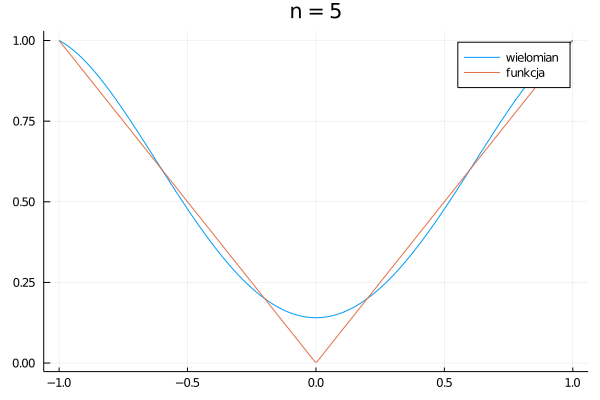
\includegraphics[scale=0.5]{z6f_5.png}
\end{figure}

\begin{figure}[h!]
    \caption{$abs(x)$ na 10 węzłach}
    \centering
    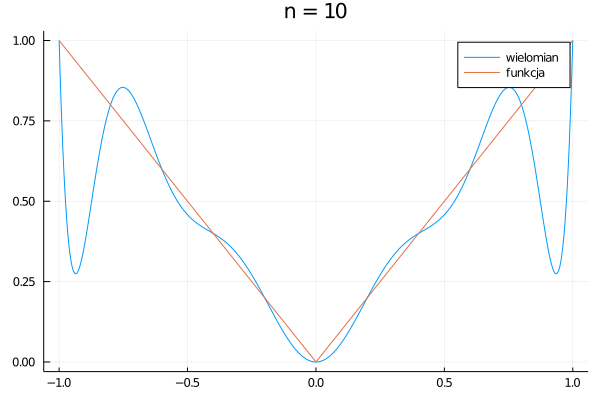
\includegraphics[scale=0.5]{popz6f_10.png}
\end{figure}
\begin{figure}[h!]
    \caption{$abs(x)$ na 15 węzłach}
    \centering
    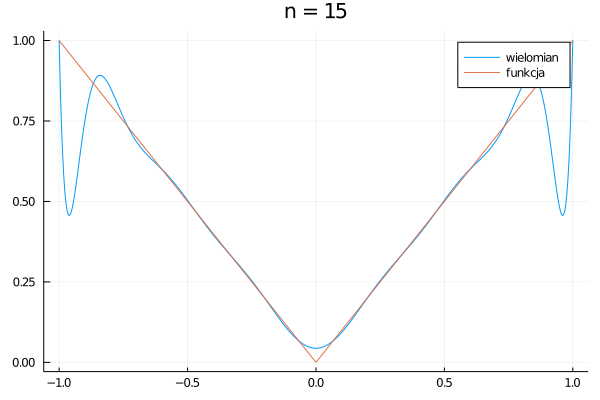
\includegraphics[scale=0.5]{z6f_15.png}
\end{figure}

\begin{figure}[h!]
    \caption{$\frac{1}{1+x^2}$ na 5 węzłach}
    \centering
    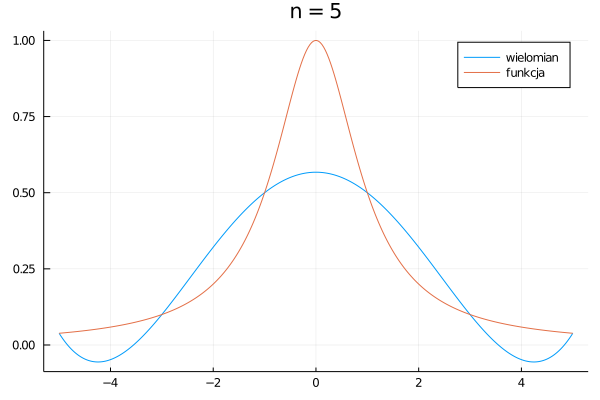
\includegraphics[scale=0.5]{z6g_5.png}
\end{figure}

\begin{figure}[h!]
    \caption{$\frac{1}{1+x^2}$ na 10 węzłach}
    \centering
    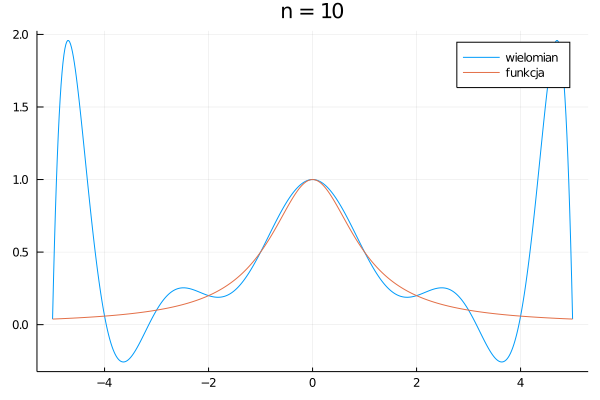
\includegraphics[scale=0.5]{popz6g_10.png}
\end{figure}
\begin{figure}[h!]
    \caption{$\frac{1}{1+x^2}$ na 15 węzłach}
    \centering
    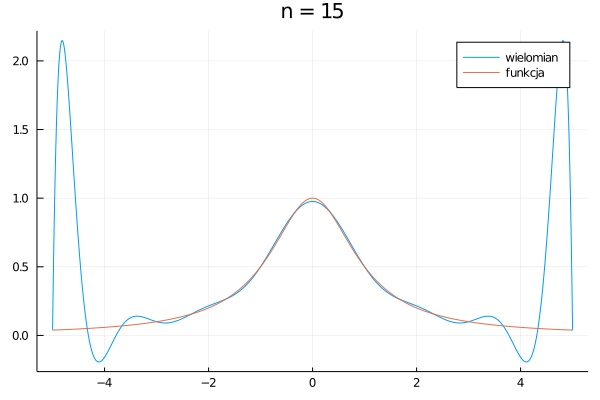
\includegraphics[scale=0.5]{z6g_15.png}
\end{figure}
\newpage
\subsection{Wnioski}
W powyższych przykładach obserwujemy dużą rozbieżnośc wielomianu interpolacyjnego z funkcją.
W pierwszym przykladzie problem wynika z nieróżniczkowalności funkcji w zerze - ma ona nienaturalny punkt złamania.
W drugim przykladzie widoczny jest efekt Runge'go w którym wielomian interpolacyjny wychodzi znacznie dalej od funkcji w pewnych punktach
w stosunku do innych. widoć to szczególnie na krańcach przedziału. Co więcej, zwiekszenie stopnia wielomianu paradoksalnie nie poprawia
przybliżenia, a pogarsza. Wynika to z nierównomiernego przyrostu funkcji na kolejnych podprzedziałach. Wielomian do interpolacji ma węzły równoodległe i właśnie to 
prowadzi do błędów aproksymacji.
Aby uniknąć tego problemu warto zastosować wielomian o węzłach zagęszczonych na krańcach przedziału. W ten sposób zagęszczenie węzłów "dusi" ucieczkę wartości wielomianu
do +/- nieskończoności. 
Taki szcególny wielomian opisał rosyjski matematyk Pafnuty Chebyshev.

\end{document}
